\begin{frame}
\centering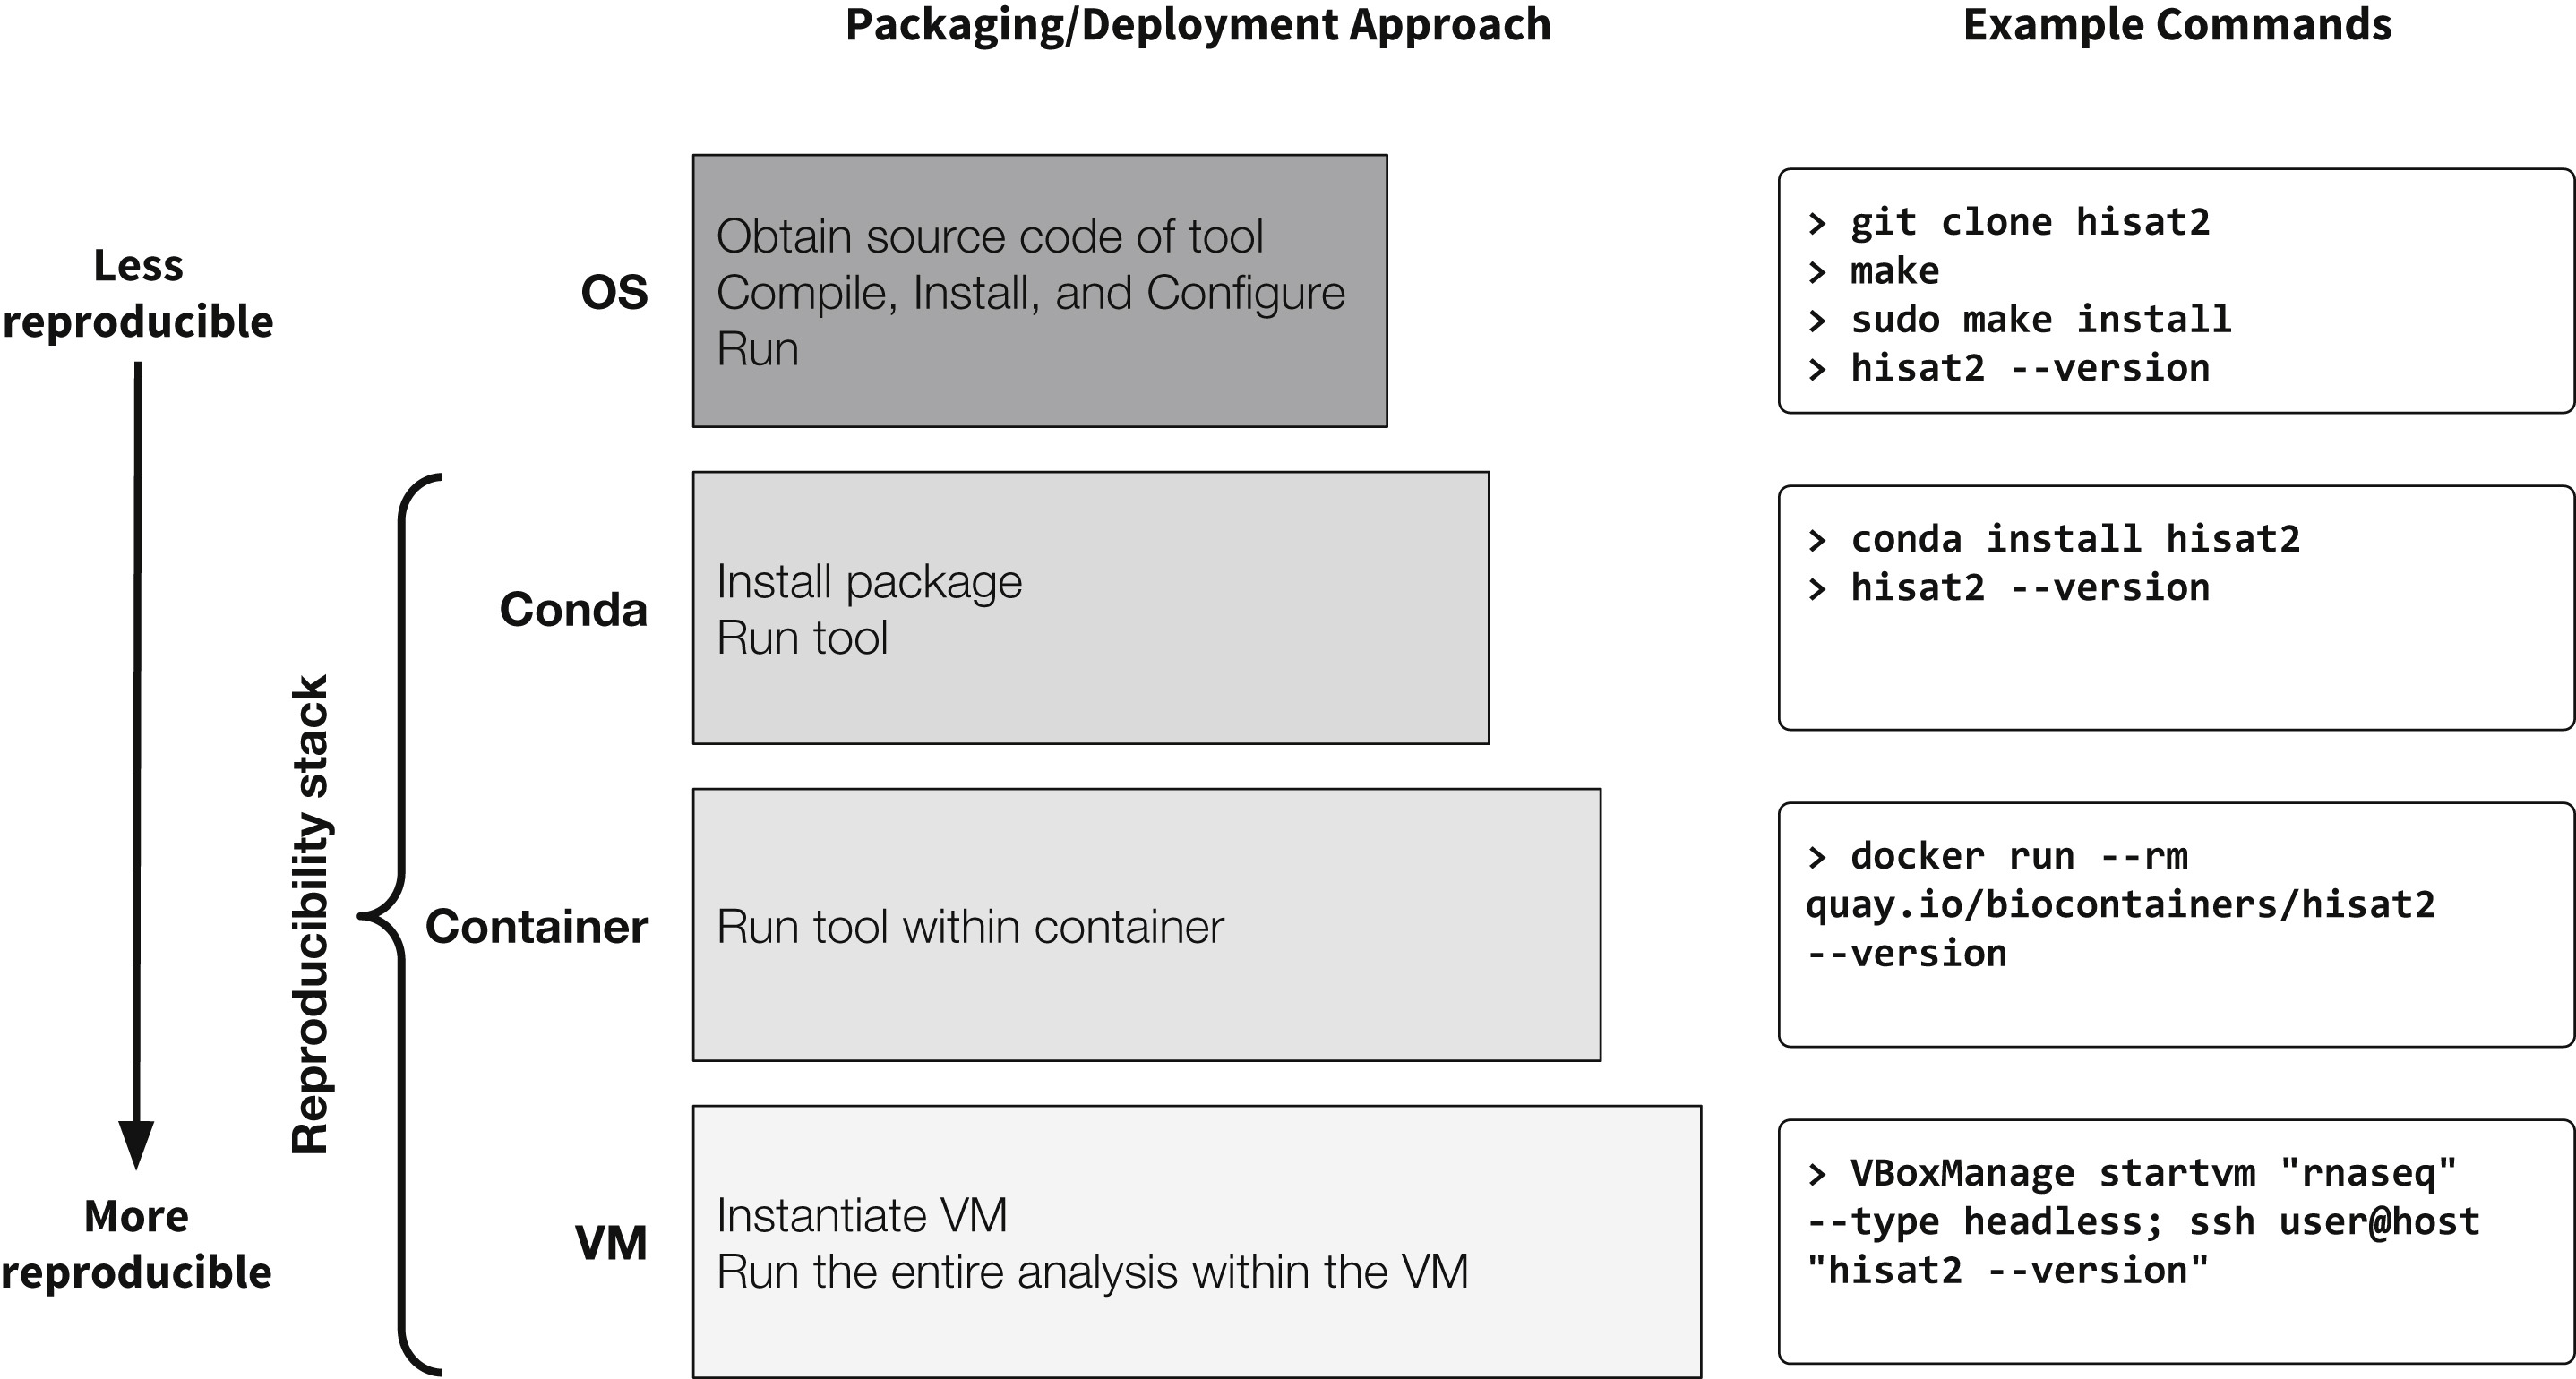
\includegraphics[width=0.8\textwidth]{images/reproductibility.jpg} \footnote{Practical Computational Reproducibility in the Life Sciences
Grüning et al, Cell Systems, 2018. DOI 10.1016/j.cels.2018.03.014}
\end{frame}
%% A METTRE EN FIN DE DIAPO
\begin{frame}[<+->]
Some recommandations \blfootnote{Recommendations for the packaging and containerizing of bioinformatics software Gruening, F1000 Research, 2019. DOI 10.12688/f1000research.15140.2}
\begin{itemize}
\item A package first
\item One tool, one container
\item Tool and container versions should be explicit
\item Avoid using ENTRYPOINT
\item Reduce the size of your container as much as possible
\item Keep data outside of the container
\item Add functional testing logic
\item Check the license of the software
\item Make your package or container discoverable
\item Provide reproducible and documented builds
\item Provide helpful usage message
\end{itemize}
\end{frame}

\begin{frame}
\begin{block}{Encapsulation PRACTICE}
\href{https://github.com/mesocentre-clermont-auvergne/formation_fair_2022/tree/main/fair_encapsulation/encapsulation_TP}{Conda and Singularity}

\end{block}
\end{frame}